
%(BEGIN_QUESTION)
% Copyright 2011, Tony R. Kuphaldt, released under the Creative Commons Attribution License (v 1.0)
% This means you may do almost anything with this work of mine, so long as you give me proper credit

Sketch the necessary tube connections to make this Fisher model DVC6000 valve positioner work with the double-acting piston actuator shown on the valve.  Two 2:1 volume boosting relays are provided for faster control valve action (for maximum of 60 PSI applied to either actuator port):

$$\includegraphics[width=15.5cm]{i02927x01.eps}$$

Assume the control valve body is direct-acting (stem {\it up} makes the valve {\it open}), and that you desire a valve action that is {\it signal-to-close} (4 mA = wide open ; 20 mA = shut).

\vfil 

\underbar{file i02927}
\eject
%(END_QUESTION)





%(BEGIN_ANSWER)

This is a graded question -- no answers or hints given!

%(END_ANSWER)





%(BEGIN_NOTES)

According to the Fisher DVD6000 manual, you need to connect the positioner's ``A'' port to the actuator's upper port, and the positioner's ``B'' port to the actuator's lower port in order to make the actuator stem extend with greater signal.  This piece of information is essential for solving the problem -- otherwise, we would be guessing which positioner port goes to which piston port.

The volume boosters require air supply just like the 30 PSI regulator, and so all air supply lines must tie together on a common ``header'' and go to the 100 PSI supply.  The ``In'' ports of the boosters need to connect to the positioner's respective ``A'' and ``B'' ports, while the ``Out'' ports of the boosters send air to and from the actuating piston.

\vskip 10pt

A useful problem-solving strategy we may apply here is to {\it simplify the problem}, in order to approach a final solution in steps.  What if we eliminate the volume boosters, connecting the positioner directly to the actuator?  This would let us figure out the proper positioner tubing without the complexity of the volume boosters getting in the way:

$$\includegraphics[width=15.5cm]{i02927x03.eps}$$

Port ``A'' on the positioner must connect to the bottom port on the piston actuator, while port ``B'' on the positioner must connect to the piston's upper port.

\filbreak

Now that we have the positioner's port connections figured out, we can connect the boosters' supply lines together to the 100 PSI header, and then insert each booster in ``series'' between each positioner output port and its respective actuator port.  Each booster will take in a pressure signal from the positioner, and then output a corresponding (2:1) air pressure to the piston actuator at high volume:

$$\includegraphics[width=15.5cm]{i02927x02.eps}$$

%INDEX% Basics, pneumatics: pressure booster
%INDEX% Final Control Elements, valve: positioner

%(END_NOTES)


